%!TEX TS-program = xelatex
%!TEX encoding = UTF-8 Unicode

% use the corresponding paper size for your ticket definition
\documentclass[letterpaper,12pt]{article}

% load fonts and graphics
\usepackage{xcolor,xifthen,xltxtra,xunicode,fontspec,epsfig}
\definecolor{RegentGrey}{HTML}{83939D}
\usepackage[pdfauthor={Testing Gravity 2015},pdftitle={Maps and Directions},colorlinks,urlcolor={RegentGrey}]{hyperref}
\defaultfontfeatures{Scale=MatchLowercase,Ligatures=TeX}

%%% Set paper size and margins
\usepackage[letterpaper]{anysize}       % Set paper size and margins
\marginsize{0.5in}{0.5in}{0.5in}{0.5in}
\setlength{\headheight}{32pt}
\setlength{\headsep}{12pt}
\flushbottom

%%% Customize layout
\usepackage{fancyhdr}
\pagestyle{fancy}
\pagestyle{fancy}
\lhead{\fontspec{Cinzel}\huge Testing Gravity 2015}\chead{}
\rhead{\fontspec{Lato Light Italic}\Large Maps and Directions}
\lfoot{}\cfoot{}\rfoot{}
%\renewcommand{\headrulewidth}{1pt}
%\renewcommand{\footrulewidth}{1pt}

% EB Garamond
\setmainfont{Lato}[ItalicFont={Lato Italic}, BoldFont={PT Sans}, BoldItalicFont={PT Sans Italic}, SmallCapsFont=Cinzel]
\setsansfont{Lato}
\setmonofont{Jura}

\usepackage{titlesec}

\titleformat*{\section}{\fontsize{24pt}{24pt}\bfseries}
\titleformat*{\subsection}{\fontsize{18pt}{18pt}\bfseries}
\titleformat*{\subsubsection}{\large\bfseries}
%\titleformat*{\paragraph}{\large\bfseries}
%\titleformat*{\subparagraph}{\large\bfseries}

\newcommand{\bus}[1]{\textit{``#1''}}

\begin{document}

\section*{Maps and Directions:}

\begin{center}
\begin{tabular}{ll}
\href{https://goo.gl/maps/9wDiq}{\Large getting there:}&
\href{https://www.google.com/maps/d/viewer?mid=zq57oNda8OcY.k02ESQNIl2-8}{\Large conference venue and neighbourhood:}\\
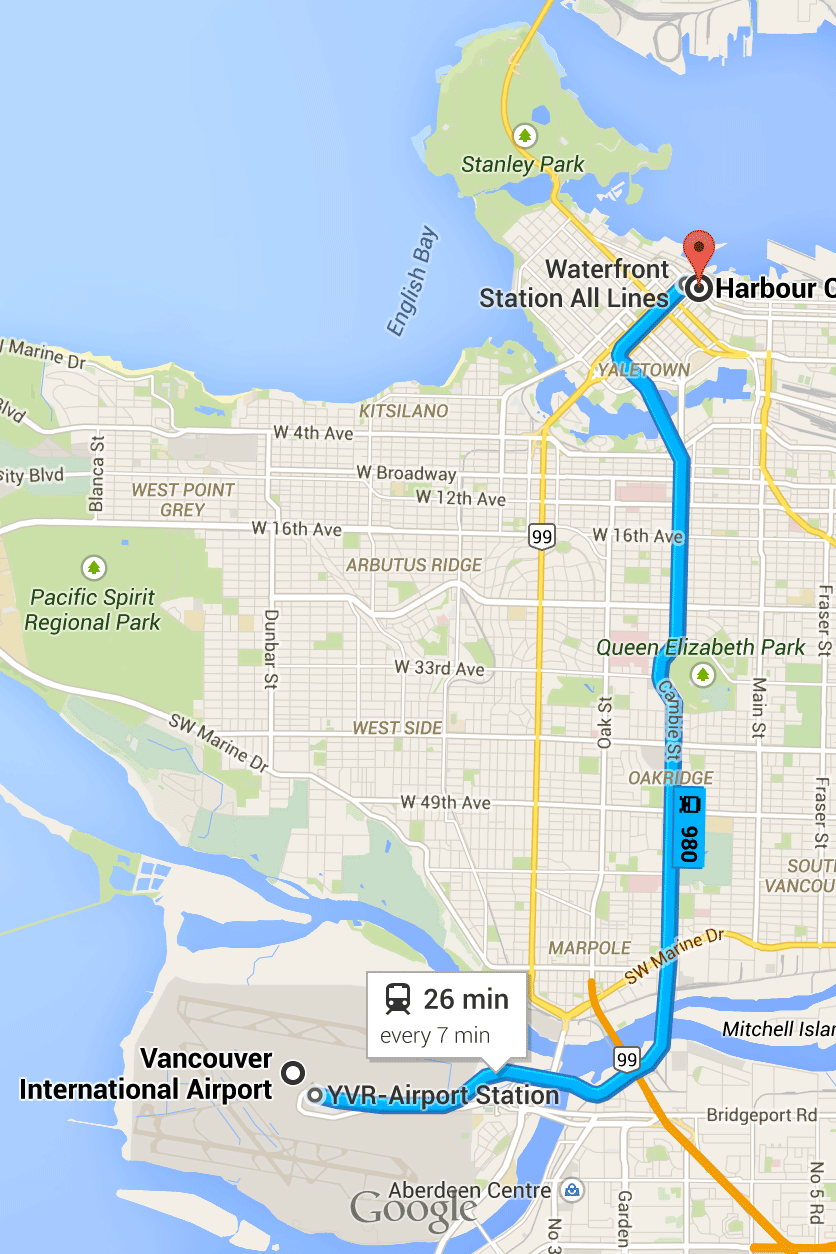
\epsfig{file=directions.png,height=3in} & 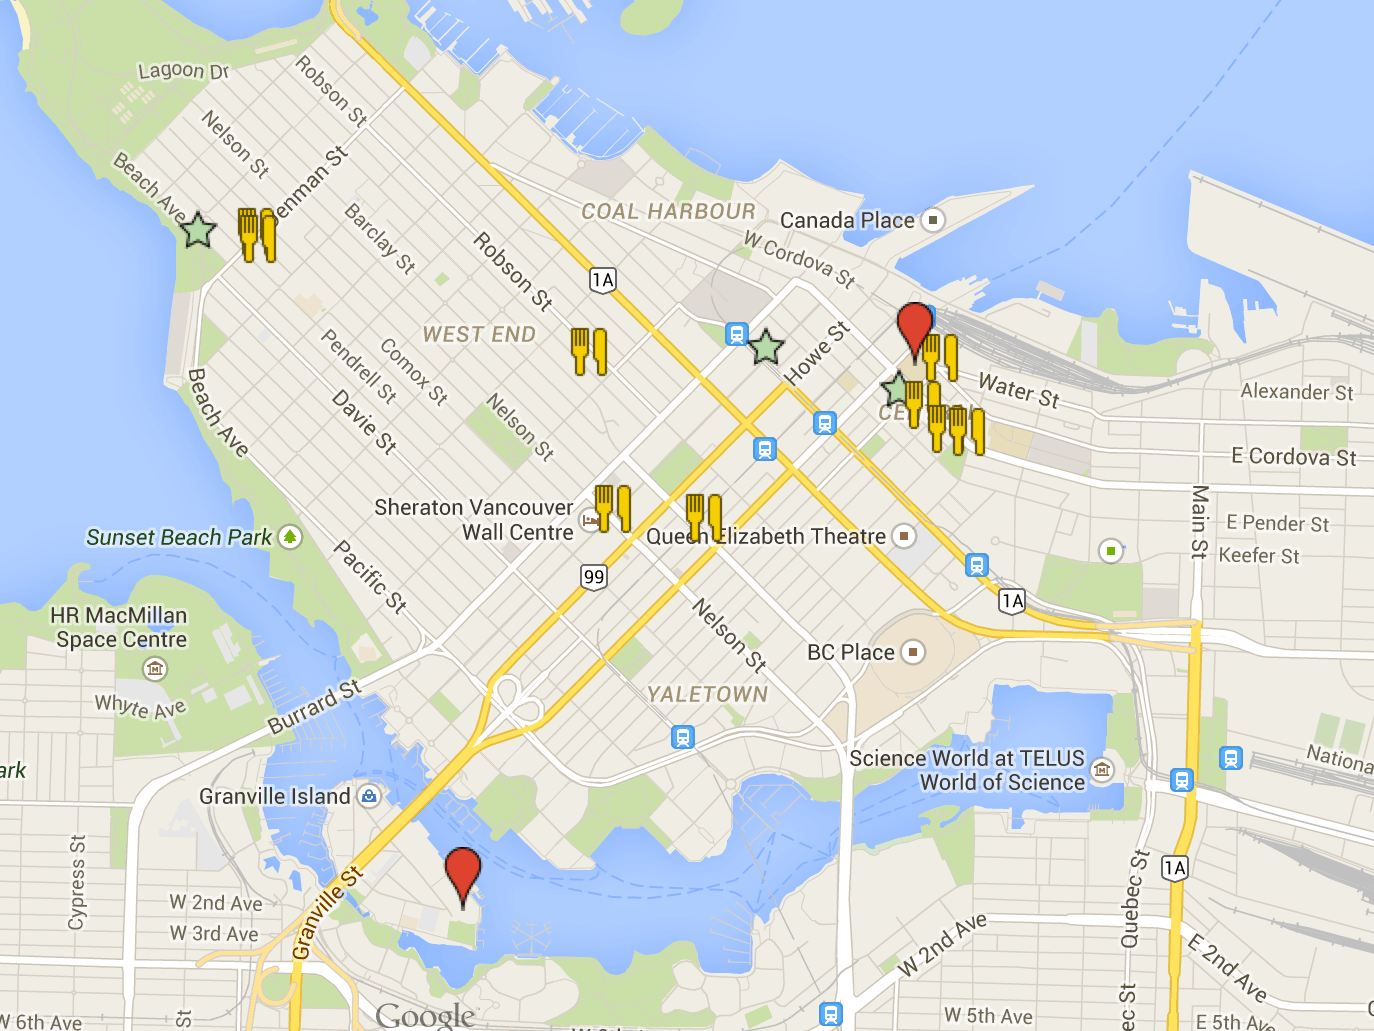
\epsfig{file=venue.png,height=3in}\\
\end{tabular}
\end{center}

\noindent
A lot of Vancouver is very walkable, and the buses are easy to use. They cost \$2.75 for a one way ticket that will allow you to take as many transfers as needed, and expire after 90 minutes. Many buses run quite late as well. Here you will find directions to walk or bus to and from the conference, as well as the banquet at 19:00 on Friday night on Granville Island. If you are in need of further directions, Google Maps provides accurate information for Vancouver transit. There are also suggestions for places to eat, and some other popular activities in Vancouver.

\section*{Getting to the Hotels:}

Please note that the registration desk will be open all day on Wednesday and Thursday until 21:00. If your flight lands before 19:00, we suggest that you follow the instructions on how to get to the workshop. You can register there and volunteers can then help you get the right bus to Sylvia Hotel, or show you how to find Delta Hotel (which is across the street).

To get onto the SkyTrain at the airport, the first step is to find the SkyTrain station just outside of the airport, there are signs, and it is just outside of the terminal. Note that taking the SkyTrain from the airport costs \$5 more than normal. You can get around this fee by purchasing prepaid fares called FareSavers at the 7-Eleven or the Pharmasave located on Level 1 in the Domestic Arrivals Terminal.

\subsection*{Delta Vancouver Suites:}

Delta hotel is right across the street from the workshop venue. Therefore, those staying at Delta have the option to easily register at the venue and then check in, or go straight to the hotel.
Take the SkyTrain all the way to Waterfront station. When you get off the train, take the exit to the right to Granville Street. When you are above ground, turn around and go right on West Hastings Street. Delta Vancouver Suites is just over one block away past the Seymour and West Hastings intersection. The entire trip should take less than 30 minutes, and the SkyTrain comes about every 6 minutes.

\subsection*{The Sylvia Hotel:}

For those staying at The Sylvia Hotel and whose flights land before 19:00, we suggest that they follow the instructions on how to get to the workshop. They can register there and volunteers can then help them catch the right bus to Sylvia Hotel.
If you are landing after 19:00, you have the option to get a taxi straight from the airport to the hotel and it will cost about \$40 CAD. The cheaper (and still relatively convenient) way is to take the SkyTrain to Yaletown-Roundhuse station and take a taxi from there. Yet, a cheaper option is to use public transit as instructed below.

Take the SkyTrain to the Yaletown-Roundhouse stop. Exit on Davie Street and walk less than a block to Davie and Mainland. Take the \bus{C21 Beach} or the \bus{C23 Davie} bus to Morton and Beach and walk back to Beach Avenue. Alternatively, you can take a taxi from Yaletown-Roundhouse. The Sylvia Hotel should be less than one block away at Beach and Gilford. The entire trip should take about 45 minutes.


\section*{Getting to the Workshop:}

\subsection*{From Delta Vancouver Suites:}

Delta Vancouver Suites faces SFU Harbour Centre on West Hastings Street and you can simply cross the street to get to the conference.

\subsection*{From the Sylvia Hotel:}

The Sylvia Hotel is not quite as close as Delta, and it is a 30 to 40 minute walk to the conference. To get to the Harbour Centre by walking, go up Gilford Street. It will turn right into Pendrell Street, and then take a left at Denman Street. Walk all the way to West Georgia Street, turn right, and then turn left on Cardero Street followed by a final right on West Hastings Street. Follow West Hastings all the way to Harbour Centre.

If instead you would like to bus, there are two bus routes that will take you very close to the conference without much walking. Both options will take 20-30 minutes. From the Sylvia Hotel, turn right onto Gilford Street, which will quickly turn into Pendrell Street. Turn left on Denman Street, and wait for the \bus{005 Downtown} bus. There should be a bus roughly every 8 minutes. Get off the bus at Hastings and Seymour, and Harbour Centre will be right there. The other option is to take a left on Beach Avenue and another left on Davie Street, and wait at the stop just past Denman Street for the \bus{006 Downtown} bus. Again, the buses arrive roughly every 8 minutes. Get off the bus at Granville and Hastings, and walk towards Seymour St. Harbour Centre is only one block away.

To get back to the hotel, the \bus{005 Robson} and the \bus{006 Davie} buses are your best options. The \bus{005 Robson} stops just outside Harbour Centre at Hastings and Seymour, and the \bus{006 Davie} stops at Richards and Hastings. Note that you will have to turn right out of Harbour Centre, and then turn right again on Richards Street to catch the \bus{006}.


\section*{Getting to the Banquet:}

There are several options for bussing from the hotels or from the conference to the banquet dinner at Dockside on Granville Island. Volunteers will be leaving periodically from Harbour Centre and can help you find your way. Walking to Granville Island is not recommended, as crossing the Granville Street bridge as a pedestrian is not ideal.

\subsection*{From Delta Vancouver Suites and Harbour Centre:}

Bussing from Delta Vancouver Suites or the Harbour Centre itself is easy. Turn right on Seymour Street and walk towards the water to West Cordova Street. Cross the street and wait for a \bus{050 False Creek} bus. Take it to West 2nd and Anderson, and then cross the bridge to Granville Island and take a right on Cartwright Street. Follow it all the way to the end to Dockside. The trip will take about 30 minutes, and the \bus{050 False Creek} comes every 15 minutes. To make it on time, take the bus at 18:19 or the bus at 18:34.

\subsection*{From the Sylvia Hotel:}

To bus from the Sylvia Hotel, you first have to get to Granville and Davie. There are two options. First, you can take a left on Beach Avenue and another left on Davie Street, and wait at the stop just past Denman Street for the \bus{006 Downtown} bus, as if going to the conference. This time, get off the bus at Granville and Davie, and then cross the street both ways. Alternatively, you can take a left on Beach Avenue and then an immediate left on Morton Avenue. Wait for the \bus{C23 Main St} and take it to Davie and Howe. Walk one more block to Granville Street and turn right.

At Granville and Davie, wait for a \bus{050 False Creek} bus, and get off at West 2nd and Anderson. Cross the bridge to Granville Island, and take a right on Cartwright Street. Follow it all the way to the end to Dockside. The trip will take about 40 minutes, and the \bus{050 False Creek} comes every 15 minutes. To make it on time, take the \bus{006} at 18:27, or the \bus{C23} at 18:25.

The other option is to take a False Creek Ferry. You can find these small passenger ferries just in front of the Vancouver Aquatic Centre of Beach Avenue, and take them one stop to Granville Island. On Granville Island, simply turn left on Johnson Street and walk all the way to the end to Dockside. You can get to the ferry by walking along Beach Avenue, which will take about 20 minutes but is a very nice walk, or by taking the \bus{C21 Yaletown} at Morton and Beach and getting off at Beach and Thurlow. The ferry costs \$3.25, or you can buy a round trip ticket for \$5.50, and they come about every 5 minutes until 21:00.


\section*{Places to Eat:}

Vancouver is an awesome city for eating out, especially for Asian food of all types, but including other international cuisine and fusion. The list below is a short-list of some of the organizers’ favourites.

\subsection*{Near Harbour Centre and Delta Vancouver Suite:}
\begin{itemize}
\setlength{\itemsep}{0pt}
\item \href{http://www.steamworks.com}{\textbf{Steamworks}}, 375 Water Street: This brew pub is a Vancouver staple. You will find all of the standard pub fare and more, and it is also a great chance to try some local award winning beer.
\item \href{http://www.bonchaz.ca}{\textbf{Bonchaz}}, 426 W Hastings Street: This small bakery has delicious sandwiches served on bread baked in house. Their claim to fame is the Bonchaz Bun, which is a sweet dough bun with a butter and sugar filling. Great for lunch.
\item \href{http://www.lataqueria.com}{\textbf{La Taqueria}}, 322 W Hastings Street: This little taco shop is home to probably the best tacos in Vancouver, and is a great stop for lunch.
\item \href{http://www.nuba.ca}{\textbf{Nuba}}, 207 W Hastings Street: This excellent Lebanese restaurant is good for lunch or dinner.
\end{itemize}

\subsection*{Near the Sylvia Hotel:}
\begin{itemize}
\setlength{\itemsep}{0pt}
\item \href{http://www.akirasushi.ca}{\textbf{Akira Sushi}}, 1069 Denman Street: An excellent choice if you are feeling like sushi.
\item \href{http://www.bananaleaf-vancouver.com}{\textbf{Banana Leaf}}, 1096 Denman Street: This award winning Malaysian restaurant serves their food tapas-style, where all dishes are shared.
\end{itemize}

\subsection*{Further Afield}
\begin{itemize}
\setlength{\itemsep}{0pt}
\item \href{http://www.shizenya.ca}{\textbf{Shizen Ya}}, 985 Hornby Street: This delicious sushi restaurant serves only brown rice, and all of their salad is made with organic vegetables. It has vegan and gluten-free options as well.
\item \href{http://www.cafecrepe.com}{\textbf{Cafe Crepe}}, 874 Granville Street: This is a great place to stop at lunch for a quick crepe.
\item \href{http://www.zefferellis.com}{\textbf{Zefferelli's}}, 1136 Robson Street: This spaghetti joint has a lovely atmosphere and is right above one of the busiest shopping streets in Vancouver.
\item \href{http://www.thenaam.com}{\textbf{The Naam}}, 2724 West 4th Avenue: This is a very busy vegetarian restaurant that is open 24 hours a day 7 days a week. They also have live music from 19:00-22:00 every night. It is a bit further away, but the trip is worth it. Make sure to try the sesame fries and miso gravy.	
\item \href{http://www.healthynoodle.ca}{\textbf{Healthy Noodle House}}, 2716 West 4th Avenue: Right next door to the Naam, this noodle house is very small, but the owner is very friendly and the food is delicious. Stop by if the Naam is too busy, or you want tasty noodle soup without high sodium or MSG.
\item \href{http://www.vijsrestaurant.ca}{\textbf{Vij's}}, 1480 W 11 Avenue: This award winning Indian restaurant serves inventive dishes and has a great atmosphere. They do not take reservations, and open at 17:30.
\end{itemize}


\section*{Things to do in Vancouver:}

\begin{itemize}
\setlength{\itemsep}{0pt}
\item \href{http://www.vancouverlookout.com/}{\textbf{Harbour Centre Tower:}} Located right above our meeting venue, the tower offers 360º aerial view of Vancouver and the surrounding area. Pretty at night! 
\item \href{http://vancouver.ca/parks-recreation-culture/seawall.aspx}{\textbf{The Seawall:}} Walk, run, or bike the Seawall, a scenic 22 km path that extends all the way from Coal Harbour downtown to Kitsilano Beach. It is a beautiful trail, especially if the weather cooperates.
\item \href{http://vancouver.ca/parks-recreation-culture/stanley-park.aspx}{\textbf{Stanley Park:}} This enormous park is very close to downtown. There are kilometers of trails, scenic views, and other things to see. TripAdvisor recently named it the top park in the world.
\item \href{http://granvilleisland.com/}{\textbf{Granville Island:}} Granville Island is one of the top tourist destinations in the city. With a mix of shops, restaurants, theatres, a market and a marina, there is something for everyone. Our banquet venue is located there.
\item \href{http://www.vanaqua.ca}{\textbf{Vancouver Aquarium:}} This aquarium is located in the heart of Stanley Park, and is the largest aquarium in Canada. It is home to two dolphins, two beluga whales, and over 50,000 different animals.
\item \href{http://moa.ubc.ca/}{\textbf{UBC Museum of Anthropology:}} This museum is probably the top world-class museum in the lower mainland, with collection consisting of 40,000 objects representing cultures from all over the world.
\item \href{http://www.flyovercanada.com}{\textbf{Fly Over Canada:}} This flight simulation ride takes you all over Canada, and is complete with scents, mist, and wind. It is located at Canada Place, quite close to Harbour Centre.
\item \href{http://www.capbridge.com/}{\textbf{Capilano Suspension Bridge:}} Check out spectacular Capilano Canyon from high above on a suspension bridge, and walk the local rainforest habitat among 1300-year-old old Douglas firs.
\item \href{http://www.grousemountain.com/}{\textbf{Grouse Mountain Gondola:}} Grouse Mountain Gondola will take you high in the North Shore mountains with spectacular views of the Vancouver. Fun even if you do not ski! Even better if you do!
\item \href{http://www.whistlerblackcomb.com/}{\textbf{Visit Whistler:}} While not in Vancouver, the resort municipality of Whistler is a very popular destination for skiing, snowboarding, and other winter activities. There are shuttles from downtown to get there.
\end{itemize}

\end{document}
